\chapter{Implementation}

\section{Creating the dataset}\label{chp:dataset}
DCNN make use of vast amounts of data for training. The MNIST dataset contains 60.000 training examples and 10.000 test examples, the Pascal VOC 2012 segmentation dataset \cite{PASCALVOC2012} has a total of 9993 segmented images, the Microsoft COCO dataset \cite{Lin2014} has over 200.000 segmented images and Google's internal JFT dataset \cite{Hinton2015} has over 300 million images with labels. There is a general agreement in the field on DCNNs that the revolution in semantic segmentation is a product of the large datasets available \cite{Sun2017}.

Most of the reviewed networks build on pre-trained models to save computational time and to focus on training the network at the task at hand. Using pre-trained networks also lowers the need to have a large dataset available. In the case of zoning regulations, there does not exist a dataset that has been used or can be used to train the network. This must, therefore, be created.

As stated in \autoref{chp:motivation}, 354 out of 426 municipalities are registered to have digital zoning registers. This implies that they have PDF's with scanned raster regulations openly available and published online. The PDF files have varying quality and some of them can be very old as seen in \autoref{fig:regulations}. Some of these municipalities also have vectorized their regulations. It can, therefore, be possible to use the already vectorized regulations to create a dataset that can be used for training the neural network.

\begin{figure}[H]
    \centering
    \includegraphics[width=\linewidth]{fig/zoning-regulations.png}
    \caption{Samples of the zoning regulations.}
    \label{fig:regulations}
\end{figure}

A problem with this is that the PDFs are not georeferenced, that is, we do not know the coordinates of the corners of the PDF. A procedure that connects the boundary of the vectorized zoning areas to the same area within the PDF is therefore needed. The problem can be seen in \autoref{fig:georeferencing} where we see the vectorized bounding area on the left and the scanned zoning regulation PDF on the right. A possible approach is to use a computer vision framework such as OpenCV \footnote{Link: https://opencv.org/} and its feature detection library to find the translation between the images. After the translation is found it would be possible to generate a training image the size of the PDF and with proper labels. This procedure does, however, add a possible source of error that has to be examined thoroughly.

\begin{figure}[H]
    \centering
    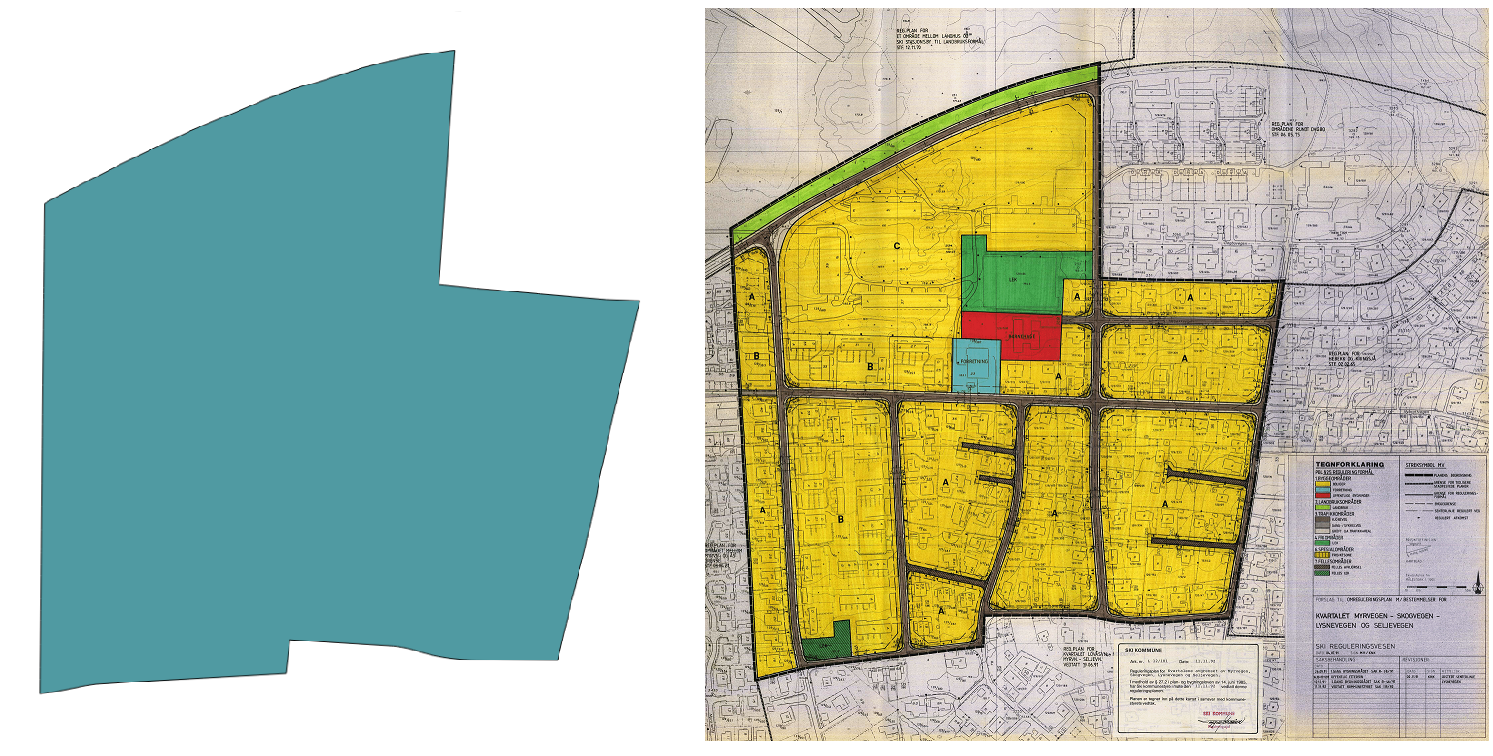
\includegraphics[width=\linewidth]{fig/georef-problem.png}
    \caption{Vectorized bounding area on the left and scanned zoning regulation og the right.}
    \label{fig:georeferencing}
\end{figure}

Another approach is to create the dataset with a micro-tasking tool, such as Amazon Mechanical Turk \footnote{Link: https://www.mturk.com/mturk/welcome}, that allows you to outsource the work on the internet. This is for instance how the Microsoft COCO and ImageNet datasets were created \cite{Lin2014}. This can, however, be a very time-consuming process as seen in the creation of COCO, where the segmentation required 22 worker hours per 1000 images. One could argue that the time spent creating the training data, could be used to vectorize the rest of the regulations instead of generating training data. When outsourcing the work, one would also need to do quality checks of the data and prepare the data so that it is an easy task for the participants to do, as they do not necessarily have any knowledge or skills regarding vectorization.

\subsection{Feature matching with OpenCV}
There was done some initial testing of feature detection with OpenCV. The method tried was brute force matching with Oriented FAST and Rotated BRIEF (ORB) descriptors with greyscale images and greyscale thresholded, contoured images. Since proper testing of multiple alternatives is outside of the scope of this paper, this cannot be viewed as absolute results.

The results from the greyscale images can be seen in \autoref{fig:test1} and as we can see, the algorithm did not manage to find any matches. The same method was tried when using contour detection first, as seen in \autoref{fig:thresh} the results did not become better.


\begin{figure}[H]
    \centering
    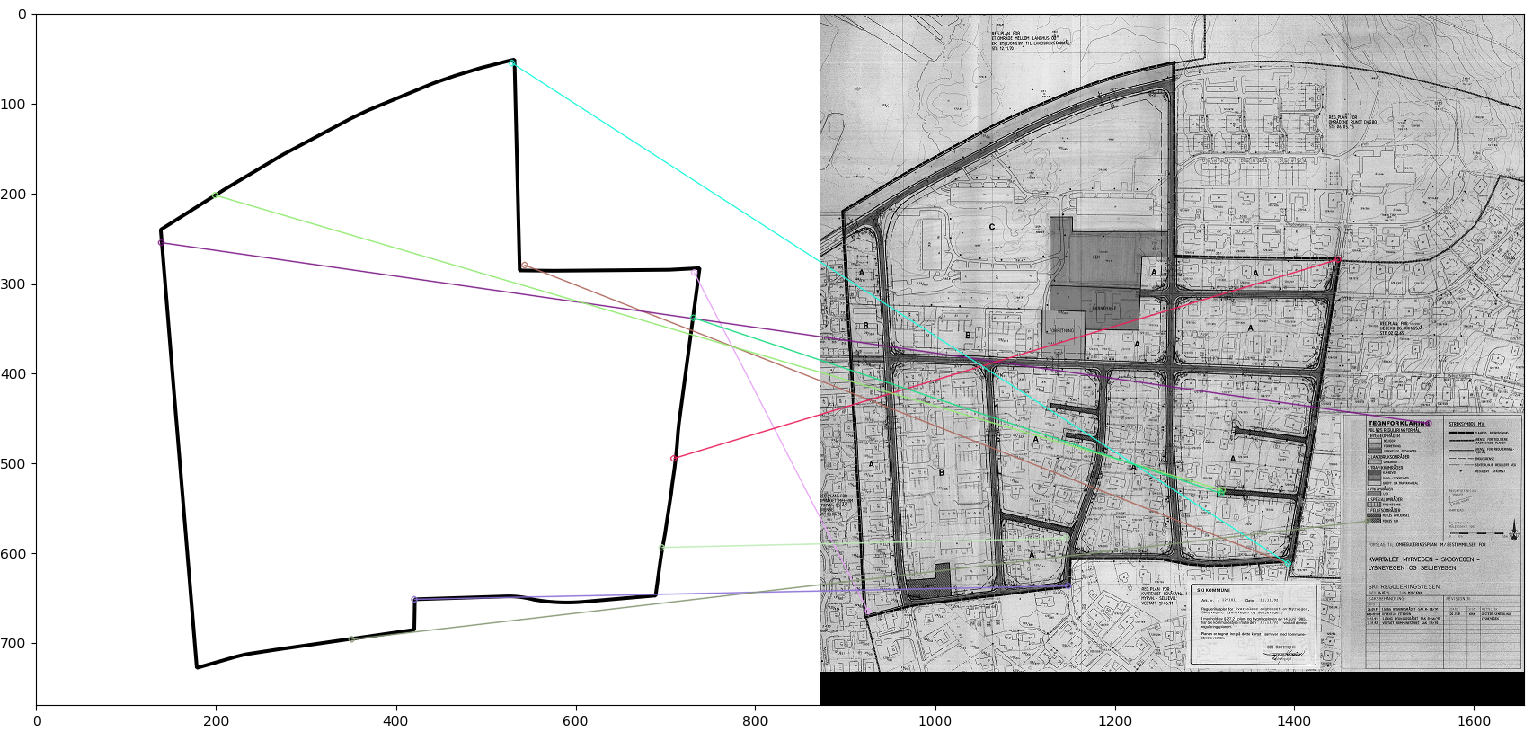
\includegraphics[width=0.8\linewidth]{fig/test1.png}
    \caption{Vectorized bounding area on the left and scanned zoning regulation og the right.}
    \label{fig:test1}
\end{figure}

\begin{figure}[H]
    \centering
    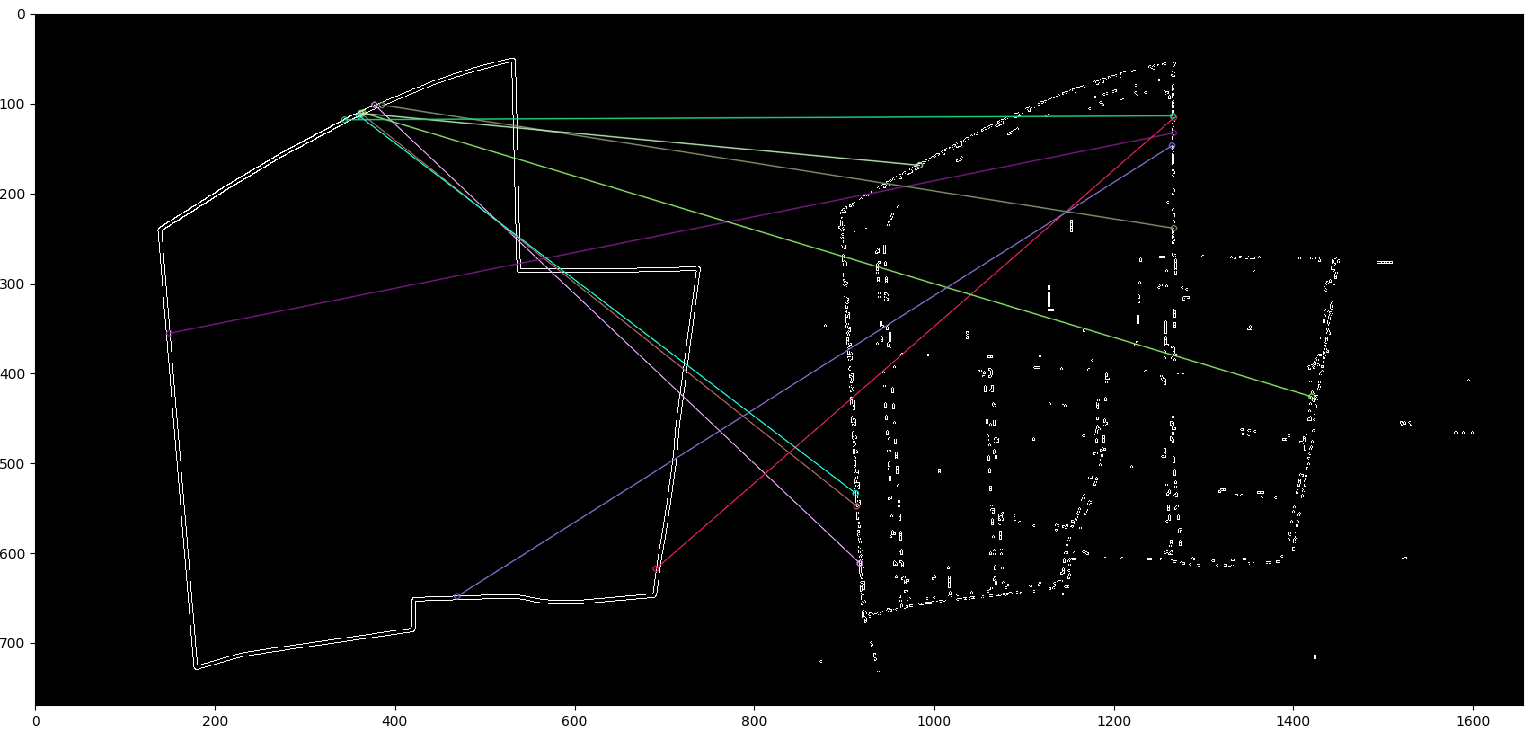
\includegraphics[width=0.8\linewidth]{fig/test1-thresh.png}
    \caption{Vectorized bounding area on the left and scanned zoning regulation og the right.}
    \label{fig:thresh}
\end{figure}

\section{Deep learning frameworks}
There exist multiple deep learning frameworks that could be used to implement the network such as Tensorflow \footnote{Link: https://www.tensorflow.org/}, Keras \footnote{Link: https://keras.io/}, CNTK \footnote{Link: https://github.com/Microsoft/cntk}, Caffe \footnote{Link: http://caffe.berkeleyvision.org/} or Torch \footnote{Link: http://torch.ch/}.  Every framework is different, some are written for a specific programming language others provide lower or higher levels of abstraction. One of the frameworks that provide the highest level of abstraction is Keras. Keras was developed with a focus on enabling fast experimentation and offers a simple API written in python. It has the ability to use either Tensorflow, CNTK or Theano (recently retired) as the underlying computation engine. With Keras, the creation of a DCNN can be done in a few lines of code and a wide variety of pre-trained networks and example architectures comes prebuilt with the framework. This makes it a good candidate for the framework to be used when implementing the network proposed in this paper. 


\section{Computational power}
Training large networks demand a considerable amount of computing power. In the early days one had to consider the cost of buying specific hardware, but with the emerge of deep learning machines in the cloud with large amounts of memory and computing power, this is not necessary anymore. As an example, the latest generation smallest computational instances on Amazon Web Services, P3.2xlarge, cost \$1.3 per Hour at the time of writing. These instances have 1 Nvidia Tesla v100 GPUs with 16 GB of GPU memory, 8 virtual CPU cores and 64 GB of ram. These instances should fit the work proposed in this paper very well.